\chapter{PoC com Containers}
\label{apendice:poc-devsecops}

Este apêndice apresenta a Prova de Conceito (PoC) desenvolvida para validação prática
do modelo de esteira DevSecOps e Infraestrutura como Código (IaC) proposto nesta
monografia.

A PoC tem como objetivo demonstrar, de forma controlada e reprodutível, a aplicação
dos conceitos, ferramentas e práticas abordadas no trabalho, simulando o
provisionamento de serviços de nuvem AWS por meio de contêineres Docker, bem como
a execução de uma pipeline automatizada com verificações de segurança e conformidade.


\section{Objetivo da Prova de Conceito}

A Prova de Conceito tem como principal objetivo validar o modelo de esteira DevSecOps
e IaC proposto, demonstrando sua viabilidade técnica e operacional em um ambiente
simulado.

Para isso, foi utilizado um ambiente baseado em contêineres Docker que simula serviços
comumente utilizados na nuvem AWS, como redes virtuais, bancos de dados relacionais
e aplicações orquestradas, permitindo a execução de todo o fluxo DevSecOps sem a
necessidade de consumo direto de recursos de nuvem pública.


\section{Visão Geral da Arquitetura Simulada}

A arquitetura da Prova de Conceito foi projetada para reproduzir, de forma simplificada,
componentes equivalentes a serviços da Amazon Web Services (AWS), possibilitando a
execução de práticas de Infraestrutura como Código e DevSecOps em ambiente local.

Os serviços simulados incluem:

\begin{itemize}
  \item VPC, representada por uma rede Docker dedicada;
  \item Amazon RDS for PostgreSQL, simulado por um contêiner PostgreSQL;
  \item Amazon EKS, representado por aplicações conteinerizadas;
  \item Elastic Load Balancer (ELB), simulado por roteamento entre serviços.
\end{itemize}

A Figura~\ref{fig:arquitetura-poc} apresenta uma visão lógica da arquitetura simulada.


% Espaço reservado para figura da arquitetura
\begin{figure}[H]
    \centering
    %\includegraphics[width=0.8\textwidth]{Figuras/arquitetura-poc.png}
    \caption{Visão lógica da arquitetura da Prova de Conceito}
    \label{fig:arquitetura-poc}
\end{figure}


\section{Ferramentas Utilizadas}

A Prova de Conceito foi desenvolvida utilizando as seguintes ferramentas, alinhadas
às práticas modernas de DevSecOps e Infraestrutura como Código:

\begin{itemize}
  \item \textbf{Terraform}: definição e provisionamento da infraestrutura simulada;
  \item \textbf{Checkov}: análise estática de segurança e conformidade do código IaC;
  \item \textbf{Git}: versionamento do código-fonte;
  \item \textbf{GitLab CI/CD}: automação da pipeline de integração e entrega contínua;
  \item \textbf{Open Policy Agent (OPA)}: validação de políticas de segurança;
  \item \textbf{Docker}: simulação de serviços de nuvem por meio de contêineres.
\end{itemize}


\section{Estrutura do Projeto}

O projeto da Prova de Conceito foi organizado de forma modular, seguindo boas práticas
de versionamento e reutilização de código. A Estrutura lógica do repositório é
apresentada a seguir:


\begin{figure}[ht]
    \caption{ Painel de incidentes e detecção de segredos do GitGuardian, apresentando a interface de monitoramento de vulnerabilidades críticas, como chaves de API e tokens expostos, permitindo a rápida remediação e mitigação de riscos de exfiltração de dados. }
    \label{fig:cvss}
    \centering
    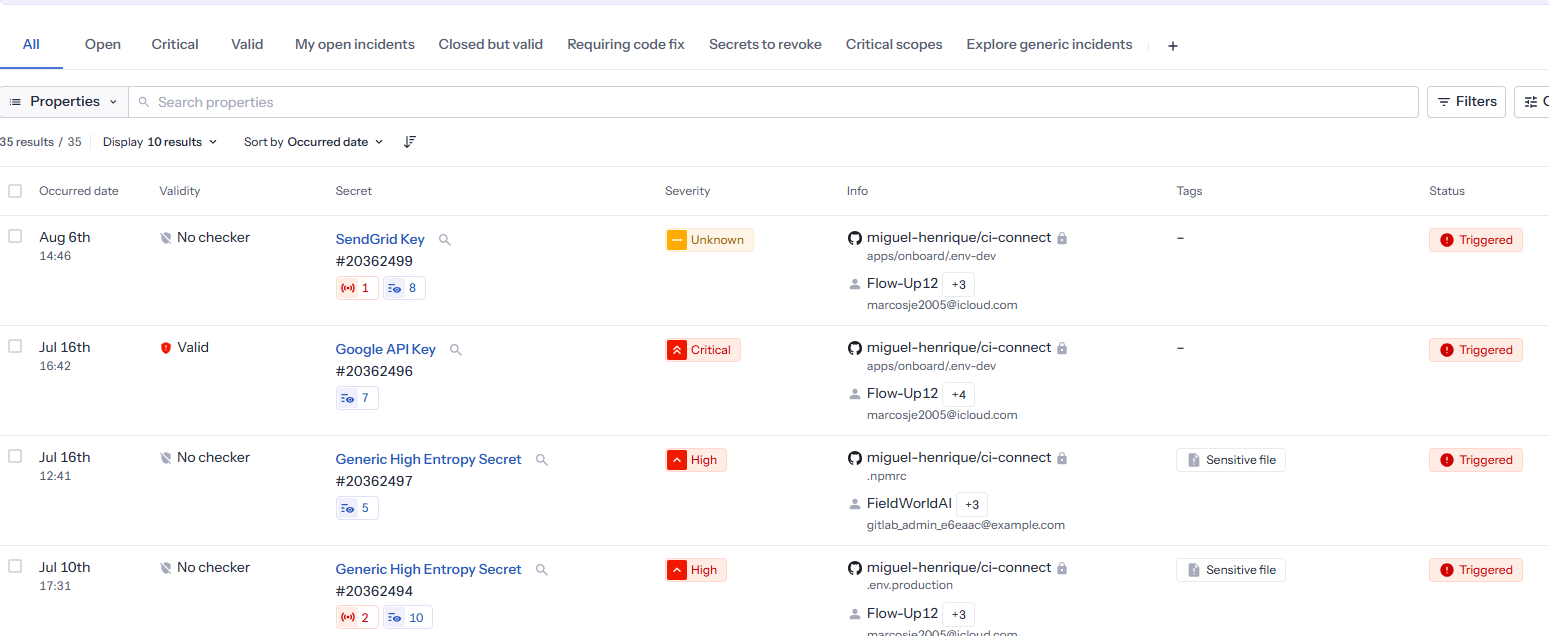
\includegraphics[width=0.8\textwidth]{Arquivos/figuras/Figura_GitGuardian_Dashboard.png}
    \fonte{Elaborado pelo autor}
\end{figure}

\begin{verbatim}
├── terraform/
│   ├── network/
│   │   └── vpc-dockernetwork.tf
│   ├── database/
│   │   └── rds-postgres.tf
│   ├── applications/
│   │   ├── eks-fastapi1.tf
│   │   └── eks-fastapi2.tf
│   └── main.tf
│
├── policies/
│   └── opa/
│       └── security.rego
│
├── scripts/
│   └── pipeline.sh
│
├── .gitlab-ci.yml
└── README.md
\end{verbatim}

\section{Pipeline DevSecOps Simulada}

A pipeline desenvolvida para a Prova de Conceito simula o fluxo completo de uma esteira
DevSecOps, integrando etapas de validação de código, análise de segurança e
provisionamento de infraestrutura.

As principais etapas da pipeline incluem:

\begin{enumerate}
  \item Validação da sintaxe e do plano de execução do Terraform;
  \item Análise de segurança do código IaC utilizando o Checkov;
  \item Avaliação de políticas de segurança por meio do Open Policy Agent (OPA);
  \item Provisionamento da infraestrutura simulada com Docker.
\end{enumerate}

\section{Evidências de Execução}

As evidências de execução da Prova de Conceito incluem o repositório de código-fonte,
os artefatos gerados pela pipeline e os resultados das ferramentas de análise de
segurança.

O repositório do projeto está disponível em:

\begin{quote}
\textbf{Repositório:} \url{<INSERIR_LINK_DO_REPOSITORIO>}
\end{quote}

\subsection{Saída da Pipeline}

A seguir são apresentados trechos da saída da pipeline DevSecOps executada durante
a Prova de Conceito.

% Espaço reservado para outputs
\begin{verbatim}
<INSERIR_OUTPUT_DO_TERRAFORM_PLAN>

<INSERIR_OUTPUT_DO_CHECKOV>

<INSERIR_OUTPUT_DO_OPA>
\end{verbatim}

\section{Considerações Finais}

A Prova de Conceito demonstrou a viabilidade técnica do modelo de esteira DevSecOps
e Infraestrutura como Código proposto nesta monografia, evidenciando que práticas
de automação, segurança e versionamento podem ser aplicadas de forma integrada,
mesmo em ambientes simulados.

Os resultados obtidos reforçam a aplicabilidade do modelo em ambientes reais de
nuvem, como a AWS, servindo como base para futuras implementações e evoluções.